\documentclass[Shifrin_Solutions_Spring_2018]{subfiles}
\begin{document}


\section{Local Theory: Frenet Frame}

%%%%%%%%%%%%%%%%%%%%%%%%%%%%%%%%%%%

\begin{exercise}
Compute the curvature of the following arclength-parametrized curves:
\begin{itemize}
\item[a.] $\alpha(s) = \left( \dfrac{1}{\sqrt{2}} \cos s , 
\dfrac{1}{\sqrt{2}} \cos s, \sin s \right)$,
\item[b.] $\alpha(s) = \left( \sqrt{1+s^2} , \ln( s + \sqrt{1+s^2} ) \right) $,
\item[c.] $\alpha(s) = \left( \dfrac{1}{3}(1+s)^{3/2} , \dfrac{1}{3}(1-s)^{3/2} , 
\dfrac{s}{\sqrt{2}} \right)$.
\end{itemize}
\end{exercise}

\begin{proof}[Solution] \begin{itemize}
\item[a.] $\kappa(s) = 1$.
\item[b.] $\kappa(s) = \dfrac{1}{1+s^2} $.
\item[c.] $\kappa(s) = \dfrac{1}{2\sqrt{2}\sqrt{1-s^2}}$.
\end{itemize}
\end{proof}

\begin{figure}[hb]
\centering
\subfloat[Ex 1(a): A circle]{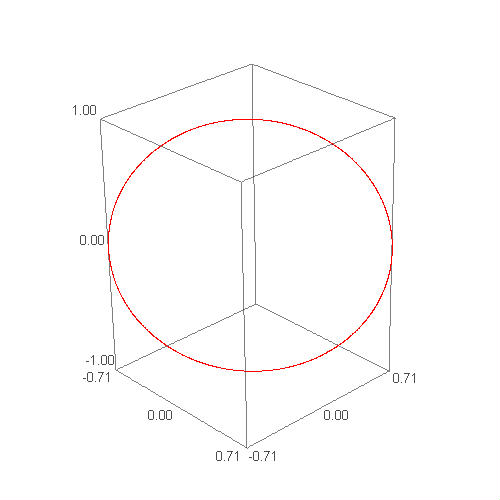
\includegraphics[width=.3\textwidth]{picturebook/ch1sec2/ex1-2-1a}}
\subfloat[Ex 1(b): Another curve]{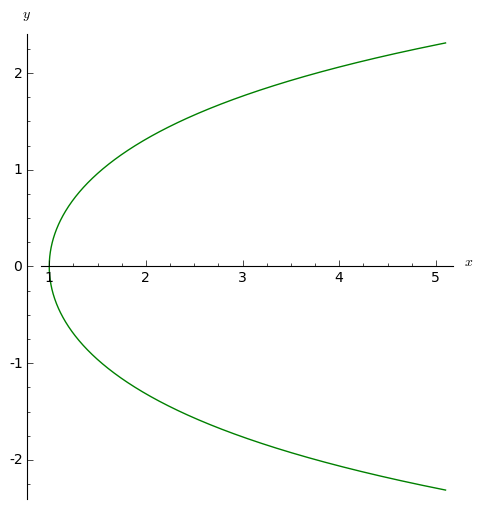
\includegraphics[width=.3\textwidth]{picturebook/ch1sec2/ex1-2-1b}}
\subfloat[Ex 1(c): And Another]{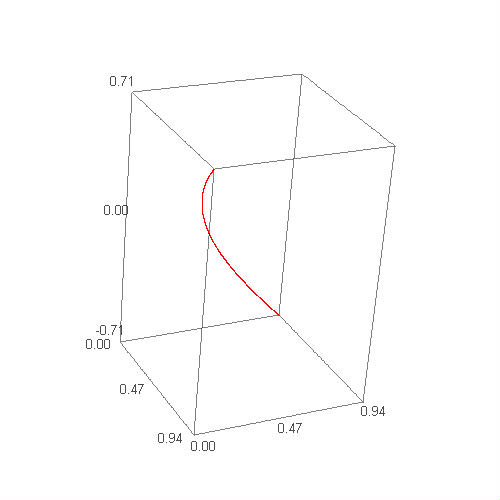
\includegraphics[width=.3\textwidth]{picturebook/ch1sec2/ex1-2-1c}}
\caption{Curves from Exercise 1}
\end{figure}

\clearpage
%%%%%%%%%%%%%%%%%%%%%%%%%%%%%%%%%%%

\begin{exercise}
Calculate the unit tangent vector, principal normal, and curvature of 
the following curves:
\begin{itemize}
\item[a.] $\alpha(t) = \left(a \cos t, a \sin t\right)$,
\item[b.] $\alpha(t) = \left( t, \cosh t \right) $,
\item[c.] $\alpha(t) = \left( \cos^3 t , \sin^3 t \right) $.
\end{itemize}
\end{exercise}

\begin{proof}[Solution]
\begin{itemize}
\item[a.]  We compute
\begin{align*}
\alpha'(t) & = \left( -a \sin t , a \cos t\right) , \\
\upsilon(t) & = a,  \\
T(t) & = (-\sin t, \cos t ) , \\
\dfrac{1}{\upsilon} \dfrac{dT}{dt} & = \dfrac{1}{a} (-\cos t, - \sin t ) , \\
\kappa(t)  & =  \dfrac{1}{a} , \\
N(t) & = (-\cos t, -\sin t) .
\end{align*}

\item[b.]  We compute
\begin{align*}
\alpha'(t) & =  ( 1, \sinh t) , \\
\upsilon(t) & = \cosh t, \\
T(t) & = ( \sech t, \tanh t) , \\
\dfrac{1}{\upsilon} \dfrac{dT}{dt} & = 
\dfrac{1}{\cosh^2 t} \left( -\tanh t , \sech t \right) , \\
\kappa(t)  & =  \dfrac{1}{\cosh^2 t} , \\
N(t) & = ( - \tanh t, \sech t ) .
\end{align*}


\item[c.]  We compute
\begin{align*}
\alpha'(t) & = (\cos^3 t, \sin^3 t) , \\
\upsilon(t) & =  3 \cos t \sin t , \\
T(t) & = ( -\cos t, \sin t) , \\
\dfrac{1}{\upsilon} \dfrac{dT}{dt} & = \left( \dfrac{1}{3 \cos t} , 
\dfrac{1}{3\sin t} \right) , \\
\kappa(t)  & =  \dfrac{1}{3\cos t \sin t}, \\
N(t) & = (\sin t, \cos t) .
\end{align*}
Note that this curve is not regular at the points where $t$ is a half-integral 
multiple of $\pi$.
\end{itemize}
\end{proof}

\begin{figure}[h]
\centering
\subfloat[Ex 2(b): The Catenary]{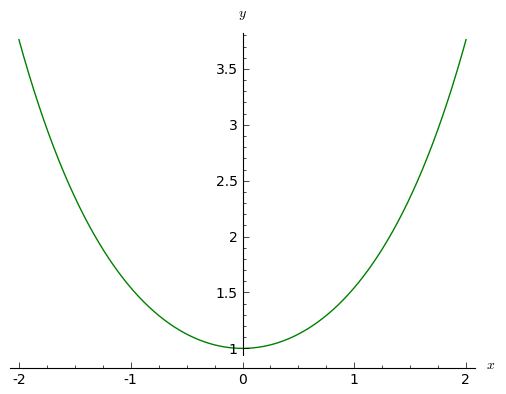
\includegraphics[width=.48\textwidth]{picturebook/ch1sec2/ex1-2-2b}}
\subfloat[Ex 2(c): An Astroid]{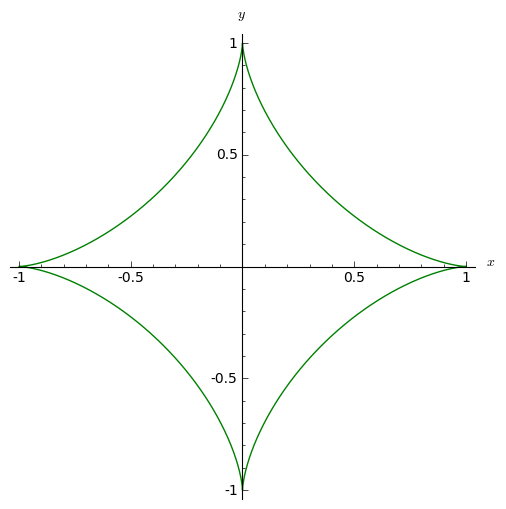
\includegraphics[width=.48\textwidth]{picturebook/ch1sec2/ex1-2-2c}}
\caption{Curves from Exercise 2}
\end{figure}

\vfill
\pagebreak

%%%%%%%%%%%%%%%%%%%%%%%%%%%%%%%%%%%

\begin{exercise}
Calculate the Frenet apparatus $(T,\kappa, N, B, \tau)$ of the following curves:
\begin{itemize}
\item[a.] $\alpha(s) = \left( \dfrac{1}{3}(1 + s)^{3/2}, \dfrac{1}{3} (1-s)^{3/2} , 
\dfrac{s}{\sqrt{2}} \right) $,
\item[b.] $\alpha(t) = \left( \dfrac{ e^t}{2} (\sin t + \cos t) ,  
\dfrac{ e^t}{2} (\sin t - \cos t) , e^t \right) $,
\item[c.] $ \alpha(t) = ( \sqrt{1 + t^2} , t , \ln(t + \sqrt{1+t^2}) )$ ,
\item[d.] $\alpha(t) = ( e^t \cos t , e^t \sin t, e^t )$,
\item[e.] $\alpha(t) = (\cosh t, \sinh t, t )$,
\item[f.] $ \alpha(t) = (t , t^2/2 , t\sqrt{1+t^2} + \ln( t + \sqrt{1+t^2})  )$,
\item[g.] $ \alpha(t) = (t - \sin t \cos t , \sin^2 t , \cos t ) $.
\end{itemize}
\end{exercise}

\begin{proof}[Solution]
\begin{itemize}
\item[a.] We compute
\begin{align*}
T(s) & =   \left(  \dfrac{1}{2}(1+s)^{1/2}  , - \dfrac{1}{2} (1-s)^{1/2} , 
\dfrac{1}{\sqrt{2}}      \right)   , \\
\kappa(s) & =  \dfrac{1}{2\sqrt{2}\sqrt{1-s^2}}  , \\
N(s) & = \dfrac{1}{\sqrt{2}} \left( \sqrt{1-s}, \sqrt{1+s}, 0 \right)    , \\
B(s) & =   \left( - \dfrac{1}{4}(1+s)^{-1/2} , - \dfrac{1}{4} (1-s )^{-1/2}  , 
0   \right)  , \\
\tau(s)  & =  \dfrac{1}{2\sqrt{2} \sqrt{1-s^2}  }   .
\end{align*}


\item[b.] We compute
\begin{align*}
T(t) & =  \dfrac{1}{\sqrt{2}} \left( \cos t, \sin t  , 1 \right)   , \\
\kappa(t) & =  \dfrac{1}{2e^t} , \\
N(t) & =   ( -\sin t , \cos t, 0)  , \\
B(t) & =    \dfrac{1}{\sqrt{2}} ( -\cos t, -\sin t, 1), \\
\tau(t)  & =   \dfrac{1}{2e^t}  .
\end{align*}

\item[c.] We compute
\begin{align*}
T(t) & =  \dfrac{1}{\sqrt{2}} \left( \dfrac{t}{\sqrt{1+t^2}} , 1 , 
\dfrac{1}{\sqrt{1+t^2}} \right)   , \\
\kappa(t) & =  \dfrac{1}{2(1+t^2)} , \\
N(t) & =  \left( \dfrac{1}{\sqrt1+t^2} , 0 , \dfrac{-t}{\sqrt{1+t^2}}      \right)   , \\
B(t) & =  \dfrac{1}{\sqrt{2}} \left( \dfrac{-t}{\sqrt{1+t^2}} , 1 , 
\dfrac{-1}{\sqrt{1+t^2}} \right) , \\
\tau(t)  & =   \dfrac{1}{2(1+t^2)} .
\end{align*}

\item[d.] We compute
\begin{align*}
T(t) & =  \dfrac{1}{\sqrt{3}} \left( \cos t - \sin t, \sin t + \cos t , 1\right)   , \\
\kappa(t) & =  \dfrac{\sqrt{2}}{3e^t} , \\
N(t) & =  \dfrac{1}{\sqrt{2}} \left( -\sin t - \cos t, \cos t - \sin t, 0 \right)  , \\
B(t) & =  \dfrac{1}{\sqrt{6}} \left( \sin t - \cos t , -\sin t - \cos t, 2 \right)  , \\
\tau(t)  & =  \dfrac{\sqrt{2}}{3e^t}  .
\end{align*}
Note that this is the same curve as that in (b) but with a different parametrization.

\item[e.] We compute
\begin{align*}
T(t) & =   \dfrac{1}{\sqrt{2}} ( \tanh t , 1, \sech t)   , \\
\kappa(t) & =  \dfrac{1}{2\cosh^2 t} \left( \dfrac{1}{\cosh t} , 0 , 
-\dfrac{\sinh t}{\cosh t} \right) , \\
N(t) & =  (\sech t, 0 -\tanh t)  , \\
B(t) & =  \dfrac{1}{\sqrt{2}}\left( -\tanh t , 1 , -\sech t \right)  , \\
\tau(t)  & =  \dfrac{1}{2} \sech^3 t  .
\end{align*}
Note that this is the same curve as in (c) but with a different parametrization.

\begin{figure}[h]
\centering
\subfloat[Curves for Ex 3b and 3d]{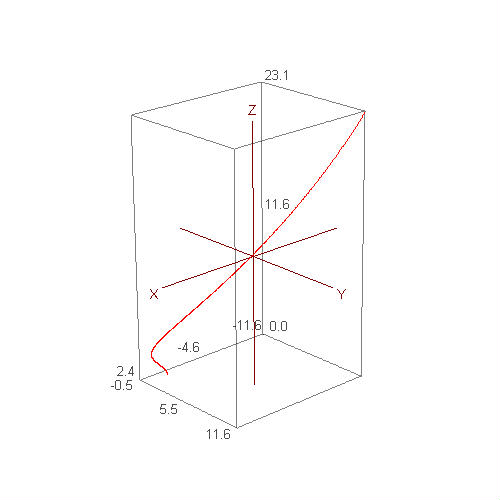
\includegraphics[width=.4\textwidth]{picturebook/ch1sec2/ex1-2-3b}}
\subfloat[Curves for Ex 3c and 3e]{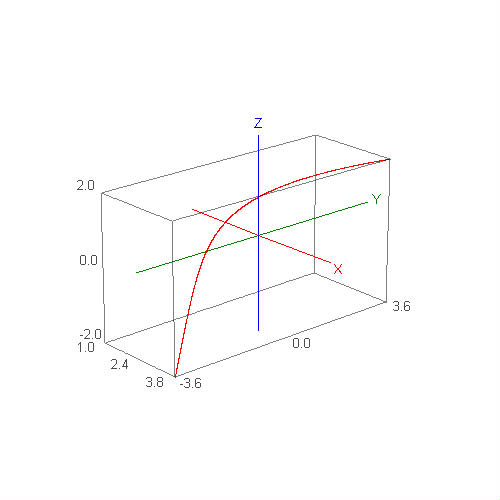
\includegraphics[width=.4\textwidth]{picturebook/ch1sec2/ex1-2-3e}}
\caption{Curves for Problem 3}
\end{figure}


\item[f.] We compute
\begin{align*}
T(t) & =  \dfrac{1}{\sqrt{5}} \left( \dfrac{1}{\sqrt{1+t^2}} , 
\dfrac{t}{\sqrt{1+t^2}} , 2 \right)   , \\
\kappa(t) & =  \dfrac{1}{5(1+t^2)^{3/2}} , \\
N(t) & =  \left( \dfrac{-t}{\sqrt{1+t^2}} , \dfrac{1}{\sqrt{1+t^2}} , 0 \right)  , \\
B(t) & =   \dfrac{1}{\sqrt{5}} \left( \dfrac{-2}{\sqrt{1+t^2}} , 
\dfrac{-2t}{\sqrt{1+t^2}} , 1 \right)  , \\
\tau(t)  & =  \dfrac{2}{5 \sqrt{1+t^2}}  .
\end{align*}

\item[g.] This time, just to be different, we slaughter an ox and offer 
up its bones in a ritual fire. In the cracked and blackened remains, our patron 
\textsc{Banjo the Clown} reveals the answers to be the ones below. Note that the 
almighty \textsc{Banjo} tells us to beware of those points where $\sin t =0$, as 
the speed vanishes at such points. Away from those stopping points, we see :
\begin{align*}
T(t) & =  \dfrac{1}{\sqrt{5}} \left( 2 |\sin t| , 2 \dfrac{\sin t}{|\sin t|} \cos t ,
 - \dfrac{\sin t}{|\sin t|} \right)   , \\
\kappa(t) & =  \dfrac{2}{5 |\sin t| }    , \\
N(t) & = \dfrac{\sin t}{|\sin t|} \left( \cos t,  - \sin t  , 0 \right) , \\
B(t) & =  \dfrac{1}{\sqrt{5}} ( -\sin t , -\cos t, -2 )  , \\
\tau(t)  & =  \dfrac{1}{5 \sin t}  .
\end{align*}
\end{itemize}
\end{proof}

\begin{figure}[h]
\centering
\subfloat[Curve for Ex 3f]{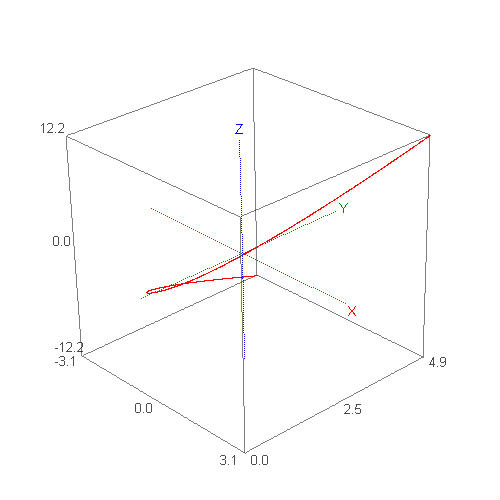
\includegraphics[width=.4\textwidth]{picturebook/ch1sec2/ex1-2-3f}}
\subfloat[Curves for Ex 3g]{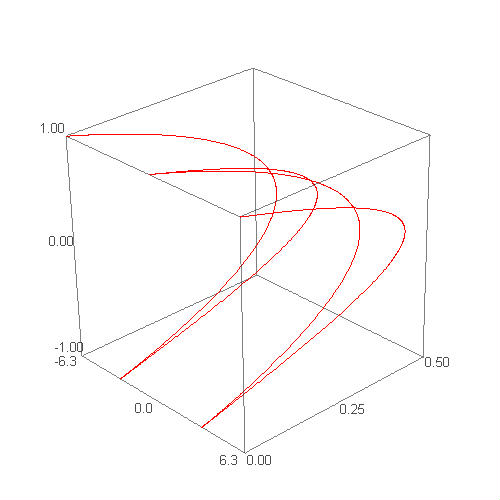
\includegraphics[width=.4\textwidth]{picturebook/ch1sec2/ex1-2-3g}}
\caption{More Curves for Problem 3 (axes not all scaled similarly)}
\end{figure}




\clearpage

%%%%%%%%%%%%%%%%%%%%%%%%%%%%%%%%%%%

\begin{exercise}
Prove that the curvature of a plane curve $y=f(x)$ is given by 
$\displaystyle \kappa = \dfrac{|f''|}{(1+(f')^2)^{3/2}}$.
\end{exercise}

\begin{proof}[Solution]
Parametrize the curve by $\sigma(t) = ( t, f(t) )$. Then we compute the following:
\begin{align*}
\sigma'(t) & = (1, f'(t) ) \\
\upsilon(t) & = \sqrt{1 + (f'(t))^2} \\
T(t) & = \left( \dfrac{1}{\sqrt{1 + (f'(t))^2} } , 
\dfrac{f'(t)}{\sqrt{1 + (f'(t))^2}} \right) \\
\dfrac{1}{\upsilon(t)} \dfrac{dT(t)}{dt} & = \ldots \\
& = \dfrac{f''(t)}{[1 + (f'(t))^2]^{3/2}} \left( \dfrac{- f'}{\sqrt{1 + (f'(t))^2}} , 
\dfrac{1}{\sqrt{1 + (f'(t))^2}} \right) .
\end{align*}
Since this last vector quantity on the right is a unit vector, it is likely 
the normal vector and the factor in front of it must be the curvature. Of course, 
curvature is positive, so we may have to change the orientation of this vector if 
$f''$ is negative. In either case, the curvature is
\[
\kappa(t) = \dfrac{|f''(t)|}{[1 + (f'(t))^2]^{3/2}}  .
\]

One can also compute this quickly using Proposition 2.2, since all we want is 
the curvature.
\end{proof}


\vspace{.5cm}

%%%%%%%%%%%%%%%%%%%%%%%%%%%%%%%%%%%

\begin{exercise}
Use Proposition 2.2 and the second parametrization of the tractrix given in 
Example 2 of Section 1 to recompute the curvature.
\end{exercise}

\begin{proof}[Solution]
The second parametrization is
\[
\beta(t) = (t-\tanh t , \sech t ), \qquad t\geq 0.
\]
By Proposition 2.2, we know that 
$\kappa = \dfrac{||\beta' \times \beta''||}{||\beta'||^3}$, so we set to computing.
\begin{align*}
\beta'(t) & = ( 1 - \sech^2 t , -\tanh t \sech t ) , \\
||\beta'(t) ||^3 & = (\tanh t)^3 , \\
\beta''(t) & = ( 2\tanh t \sech^2 t , -\sech^3 t + \tanh^2 t \sech^2 t ) , \\
\beta'(t) \times \beta''(t) &= \ldots = (0,0, \tanh^2 t \sech t ) , \\
||\beta'(t) \times \beta''(t)|| & = \tanh^2 t \sech t .
\end{align*}
Therefore, we deduce that $\kappa(t) = \csch t$.
\end{proof}

\clearpage

%%%%%%%%%%%%%%%%%%%%%%%%%%%%%%%%%%%

\begin{exercise}
By differentiating the equation $ B = T\times N$, derive the equation $B' = -\tau N$.
\end{exercise}

\begin{proof}[Solution]
Following the directions, we find this:
\[
\begin{split}
B' &= T \times N' + T' \times N \\
& = T \times (-\kappa T + \tau B) + (\kappa N) \times N \\
& = 0 + \tau (T\times B) + 0 = -\tau N.
\end{split}
\]
\end{proof}

%\vspace{.5cm}

%%%%%%%%%%%%%%%%%%%%%%%%%%%%%%%%%%%

\begin{exercise}
Suppose that $\alpha$ is an arclength-parametrized curve with the property that 
$||\alpha(s)|| \leq ||\alpha(s_0)|| =R$ for all $s$ sufficiently close to $s_0$. 
Prove that $\kappa(s_0)\geq 1/R$.
\end{exercise}

\begin{proof}[Solution]
Consider the function $f(s) = ||\alpha(s)||^2$. By our hypothesis, this function 
has a local maximum of $R^2$ at $s = s_0$. Therefore, $f''(s_0) \leq 0$. Using that 
the curve is arclength-parametrized and the Cauchy-Schwarz inequality, we compute that
\[
\begin{split}
0 & \geq f''(s_0)\\
	& = 2 \alpha'(s_0) \cdot \alpha'(s_0) + 2 \alpha(s_0) \cdot \alpha''(s_0) \\
	& = 2 \left( 1 + \kappa(s_0) (\alpha(s_0)\cdot N(s_0)) \right) \\
	& \geq 2 \left( 1 + \kappa(s_0) ( -||\alpha(s_0)||) \right) \\
	& \geq 2 \left( 1 - R \kappa(s_0) \right) .
\end{split}
\]
So, we see that
\[
\kappa(s_0) \geq 1/R .
\]
\end{proof}

\clearpage

%%%%%%%%%%%%%%%%%%%%%%%%%%%%%%%%%%%

\begin{exercise}
Let $\alpha$ be a regular (arclength-parametrized) curve with non-zero curvature. 
The normal line to $\alpha$ at $\alpha(s)$ is the line through $\alpha(s)$ with 
direction vector $N(s)$. Suppose that all the normal lines to $\alpha$ pass through 
a fixed point. What can you say about the curve?
\end{exercise}

\begin{proof}[Solution]
The condition in the problem means that there is a scalar function $\lambda$ such 
that $\alpha(s)  + \lambda(s)N(s) = P$, where $P$ is the point in question. We 
differentiate this equation to find
\[
\begin{split}
0 & = \alpha' + \lambda'N + \lambda N' \\
	& = T + \lambda' N + \lambda (-\kappa T +\tau B ) \\
	& = (1-\lambda\kappa) T + \lambda' N + \lambda\tau B
\end{split}
\]
Since $\{ T, N, B \}$ forms an orthonormal basis at each point, we see that
\begin{align*}
\kappa & = 1/\lambda , \\
\lambda' & = 0, \\
\lambda\tau & = 0 .
\end{align*}
The second equation means that $\lambda$ is constant. If $\lambda$ is always zero, 
then the curve would be stationary at $P$, and would not have normal lines, so we 
discard this case. Thus $\lambda \neq 0$. By the first equation, we see that $\kappa$ 
is constant, too. Finally, the third equation means that $\tau =0$. Hence $\alpha$ is a 
planar circle by Proposition 2.4.
\end{proof}

\clearpage

%%%%%%%%%%%%%%%%%%%%%%%%%%%%%%%%%%%

\begin{exercise}There are two independent parts.
\begin{itemize}
\item[a.] Prove that if all the normal planes of a curve pass through a particular 
point, then the curve lies on a sphere.
\item[b.] Prove that if all the osculating planes of a curve pass through a particular 
point, then the curve is planar.
\end{itemize}
\end{exercise}

\begin{proof}[Solution] We shall assume without loss of generality that the curves in 
this problem have been parametrized by arclength.
\begin{itemize}
\item[a.]  The condition means that we have a point $P$ and scalar functions $\lambda$, 
$\mu$ such that $P = \alpha(s) + \lambda(s) N(s) + \mu(s) B(s)$.
Playing with a simple example or two, it seems that we want $P$ to be the center of the 
sphere. Consider the function $f(s) = ||\alpha(s) - P||$.
Differentiating, we find
\[
\begin{split}
f'(s) / 2 & = (\alpha(s) - P) \cdot \alpha'(s) \\
	&= (- \lambda N -\mu B) \cdot T \\
	& = 0
\end{split}
\]
Thus $f(s)$ is a constant, and $\alpha$ must lie on a sphere centered at $P$. \\

\item[b.] Again, we translate our condition into a statement using the Frenet frame:
$P = \alpha(s) + \lambda(s) T(s) + \mu(s) N(s)$, and differentiate:
\[
\begin{split}
0 & = \alpha' + \lambda' T + \lambda T' + \mu' N + \mu N' \\
	& = T + \lambda' T + \lambda ( \kappa N) + \mu' N + \mu ( -\kappa T + \tau B) \\
	& = (1+\lambda' - \mu \kappa ) T + (\lambda \kappa + \mu') N + (\mu \tau) B .
\end{split}
\]
Again, we have that the Frenet frame is an orthonormal basis at each point, so 
$\mu\tau \equiv 0$. If $\mu \equiv 0$ on any interval, then the curve lies in a 
single line and the osculating planes are not defined.
Therefore, we must have that $\tau \equiv 0$, which means that $\alpha$ is 
planar by Proposition 2.4.
\end{itemize}
\end{proof}

\clearpage

%%%%%%%%%%%%%%%%%%%%%%%%%%%%%%%%%%%

\begin{exercise}
Prove that if $\kappa = \kappa_0$ and $\tau = \tau_0$ are non-zero constants, 
then the curve is a (right) circular helix.
\end{exercise}

\begin{proof}[Solution]
Without loss of generality, we assume that $\alpha$ is parametrized by arclength. 
Frenet's equation for $N$ tells us that  $N' = -\kappa_0 T + \tau_0 B$. We 
differentiate this to find:
\begin{align*}
N'' & = -\kappa_0 T' + \tau_0 B' \\
	& = -\kappa_0 (\kappa_0 N) + \tau_0 (-\tau_0 N) \\
	& = -(\kappa_0^2 + \tau_0^2 ) N .
\end{align*}
This means that $N$ satisfies the second order differential equation $N'' + k^2 N = 0$, 
where $k = \sqrt{(\kappa_0^2 + \tau_0^2 )}$. This is a simple harmonic oscillator 
equation, and its solutions are combinations of $\cos(k s)$ and $\sin(k s)$. Therefore, 
for some appropriate choice of vectors $v$ and $w$, we have
\[
\alpha''(s) = \kappa_0 N(s) = \kappa_0 \cos(ks) v + \kappa_0 \sin(ks) w .
\]
We integrate this twice to find that there are constant vectors $c$ and $b$ such that
\[
\alpha(s) = -\dfrac{\kappa_0}{k^2}\left( \cos(ks) v + \sin(ks) w \right) + s c + b .
\]
We now check that this is indeed a right circular helix. We want to show that the 
vectors $v, w$ are an orthonormal set and that $c$ is orthogonal to both $v$ and $w$. 
If this is the case, then our curve is a helix that has been hit with a rigid motion. 
The key fact is that $||N|| = 1$. Thus,
\[
1 = ||N||^2 = \cos^2(ks) ||v||^2 + \sin^2(ks) ||w||^2 + 2 \cos(ks)\sin(ks) v\cdot w.
\]
At $s=0$ we deduce that $1 = ||v||^2$. At $s = \pi/2k$, we deduce that $1 = ||w||$. 
Thus $v$ and $w$ are unit vectors. Putting this back into the equation above, we find 
that $1 = 1 + 2\cos(ks)\sin(ks) v\cdot w$.
This is only possible when $v\cdot w = 0$, so $v$ and $w$ are orthogonal. To see that 
$c$ is orthogonal to $v$ and $w$, we proceed similarly, based on the fact that $\alpha'$ 
and $N$ should be orthogonal. Using what we already know, we find  
$0 = \alpha' \cdot N = \dots = \cos(ks) c\cdot v + \sin(ks) c \cdot w.$ So, again 
choosing special values of $s$ we get the conclusion.
\end{proof}

\clearpage

%%%%%%%%%%%%%%%%%%%%%%%%%%%%%%%%%%%

\begin{exercise}
Proceed as in the derivation of Proposition 2.2 to show that
\[
\tau = \dfrac{\alpha'\cdot (\alpha''\times\alpha''')}{||\alpha' \times \alpha''||^2} .
\]
\end{exercise}

\begin{proof}[Solution]
We proceeded by computing the expression on the right. Since $\alpha$ is not necessarily 
parametrized by arclength, we denote its speed by $\upsilon$ and then
\begin{align*}
\alpha'(t) & = \upsilon T ,\\
\alpha''(t) & = \upsilon' T + \upsilon T' \\
	& = \upsilon' T + \upsilon( \upsilon \kappa N) \\
	& = \upsilon' T + \upsilon^2 \kappa N ,\\
\alpha'''(t) & = \dots \text{similar computation}\dots \\
	& = ( \upsilon''  - \upsilon^3\kappa^2  )T 
	+ ( 3\upsilon \upsilon' \kappa + \upsilon^2\kappa' ) N + (\upsilon^2 \kappa\tau ) B .
\end{align*}
Since we are going to compute the dot product of $\alpha'' \times \alpha'''$ with $\alpha' 
= \upsilon T$, we need only its $T$ component.
\[
\begin{split}
\alpha''\times \alpha''' & = (\upsilon^2 \kappa N + 
  (\text{stuff}) T) \times ( \upsilon^3 \kappa \tau B + 
  (\text{stuff}) T + (\text{more stuff}) N )\\
 & = \upsilon^5 \kappa^2 \tau T + (\text{stuff})N + (\text{stuff})B 
\end{split}
\]
So, now we follow the routine to compute that
\begin{align*}
\alpha' \cdot ( \alpha''\times \alpha''') & = \upsilon^6 \kappa^2 \tau , \text{ and}\\
||\alpha' \times \alpha''|| & = \upsilon^3 \kappa .
\end{align*}
Now it is clear that the fraction we compute will be equal to $\tau$.
\end{proof}

\vspace{.5cm}

%%%%%%%%%%%%%%%%%%%%%%%%%%%%%%%%%%%

\begin{exercise}
Let $\alpha$ be a $\mathcal{C}^4$ arclength-parametrized curve with $\kappa \neq 0$. 
Prove that $\alpha$ is a generalized helix if and only if 
$\alpha''\cdot(\alpha'''\times\alpha^{(\mathrm{iv})}) = 0$.
\end{exercise}

\begin{proof}[Solution]
Since $\alpha$ is parametrized by arclength, we can find that
\begin{align*}
\alpha' & = T ,\\
\alpha'' & = \kappa N ,\\
\alpha''' & = -\kappa^2 T +  \kappa' N + \kappa\tau B , \\
\alpha^{\mathrm{(iv)}} & = (-3\kappa \kappa') T 
 + (-\kappa^3 + \kappa''  - \kappa \tau^2 ) N 
 + (2\kappa'\tau + \kappa \tau') B.
\end{align*}
As in the last problem, we only need to find the $N$ component of 
$\alpha'''\times \alpha^{\mathrm{(iv)}}$, and this makes the next line a bit 
less cumbersome to find:
\[
\alpha''\cdot (\alpha''' \times \alpha^{\mathrm{(iv)}} ) = 
\kappa^3 ( \kappa \tau' - \kappa' \tau ) .
\]
Since $\kappa \neq 0$, we deduce that this quantity vanishes if and only if 
$\kappa \tau' - \kappa' \tau = 0$. But this is the numerator of
$(\tau/\kappa)'$. This makes it clear that 
$\alpha''\cdot(\alpha'''\times\alpha^{(\mathrm{iv})}) = 0$ if and only if 
$\tau/\kappa$ is a constant. So we are done by Proposition 2.5.
\end{proof}

\clearpage

%%%%%%%%%%%%%%%%%%%%%%%%%%%%%%%%%%%

\begin{exercise}
Suppose that $\kappa\tau \neq 0$ at $P$. Of all the planes containing the tangent 
line to $\alpha$ at $P$, show that $\alpha$ lies \emph{locally} on both sides only 
of the osculating plane.
\end{exercise}

\begin{proof}[Solution]
Without loss of generality, $P= 0$ and $\alpha$ is parametrized by arclength. Then 
by the local normal form for space curves, we have that to third order
\[
\alpha(s) = \left(s - \dfrac{\kappa_0}{6} s^3 \right) T(0) 
+ \left( \dfrac{\kappa_0}{2}s^2 + \dfrac{\kappa'_0}{6} s^3\right) N(0) 
+ \left( \dfrac{\kappa_0\tau_0}{6} s^3 \right) B(0) .
\]
A plane $\mathcal{P}$ which contains the tangent line to $\alpha$ at $P$ must have 
the form $v^{\perp}$, where $v = a N + b B$. That is, a vector $x$ lies in 
$\mathcal{P}$ if and only if $
x \cdot v = 0$. But, we can see that, to third order,
\[
(a N + b B ) \cdot \alpha(s) = \dfrac{a\kappa_0}{2} s^2 
+ \left( \dfrac{a\kappa'_0 + b\kappa_0 \tau_0}{6} \right) s^3 .
\]
For small enough $s$, this will only take one sign unless $a=0$. This gives the result.
\end{proof}

%\clearpage
\vspace{.5in}
%%%%%%%%%%%%%%%%%%%%%%%%%%%%%%%%%%%

\begin{exercise}
Let $\alpha$ be a regular curve with $\kappa \neq 0$ at $P$. Prove that the planar 
curve obtained by projecting $\alpha$ into its osculating plane at $P$ has the same 
curvature at $P$ as $\alpha$.
\end{exercise}

\begin{proof}[Solution]
This is another application of the local form. In all that we do, we shall drop terms 
of order 4 or higher in $s$. The local form of the projected curve becomes
\[
\beta(s) = \left(s - \dfrac{\kappa_0}{6} s^3 \right) T_{\alpha}(0) 
+ \left( \dfrac{\kappa_0}{2}s^2 + \dfrac{\kappa'_0}{6}s^3 \right) N_{\alpha}(0) .
\]
Here, all of the terms on the right are geometric quantities associated to $\alpha$. 
This means in particular that $s$ may not be the arclength parameter of $\beta$.
We compute that
\[
\beta'(s) = \left( 1 - \dfrac{\kappa^2}{2}s^2\right) T + \left( \kappa s 
+ \dfrac{\kappa'}{2}s^2\right) N,
\]
where $T, N, \kappa, \kappa'$ represent the values of the tangent, normal, curvature 
and derivative of the curvature of $\alpha$ at $s=0$. Since $\{T, N\}$ is an 
orthonormal basis of the osculating plane, we see that the speed of $\beta$ is given by
\[
\upsilon_{\beta}^2 = ||\beta'(s)||^2 = \dots = 1 + \kappa\kappa' s^3 + \dfrac{\kappa^4 
+ {\kappa'}^2}{4}s^4 .
\]
It is clear from this expression that $\upsilon_{\beta}(0) = 1$ and 
$d\upsilon_{\beta}^2/ds = 0$. Since 
$d\upsilon_{\beta}^2/ds = 2\upsilon_{\beta} \upsilon_{\beta}'$, we deduce that 
$\upsilon_{\beta}'(0) = 0.$
Now, if we differentiate $\beta$ in the generic way, we have $\beta' = 
\upsilon_{\beta} T_{\beta}$ and
\[
\beta'' = \upsilon_{\beta}' T_{\beta} + \upsilon_{\beta}T_{\beta}' = 
\upsilon_{\beta}' T_{\beta} + \upsilon_{\beta}\kappa_{\beta}N_{\beta} .
\]
Therefore,
\begin{equation}\label{eq:ex1-2-14--eq1}
\beta''(0) =  \kappa_{\beta}(0) N_{\beta}(0).
\end{equation}
However, if we go back to the local normal form and differentiate again, we see that
\begin{equation}\label{eq:ex1-2-14--eq2}
\beta''(s) = \kappa N
\end{equation}
Since $\kappa$ and $\kappa_{\beta}$ are both positive and $N$ and $N_{\beta}$ are 
unit vectors, we put equations (\ref{eq:ex1-2-14--eq1}) and (\ref{eq:ex1-2-14--eq2}) 
to see that $\kappa_{\beta}(0) = \kappa$. That is, the curvatures of $\alpha$ and 
$\beta$ are equal at $s=0$.
\end{proof}

\vspace{.5in}

%%%%%%%%%%%%%%%%%%%%%%%%%%%%%%%%%%%
\begin{exercise}
A closed planar curve $C$ is said to have \emph{constant breadth} $\mu$ if the distance 
between parallel tangent lines to $C$ is always $\mu$. Assume for the rest of this problem 
that the curve is arclength parametrized by a $\mathcal{C}^2$ function 
$\alpha:[0,L]\rightarrow \mathbb{R}^2$ with $\kappa\neq 0$. To say $C$ is closed means 
$\alpha(0) = \alpha(L)$ and the derivatives match as well.
\begin{itemize}
\item[a.] Let's call two points with parallel tangent lines ``opposite." Prove that if $C$ 
has constant breadth $\mu$, then the chord joining opposite points is normal to the curve 
at both points.
\item[b.] Prove that the sum of the reciprocals of the curvature of opposite points is 
equal to $\mu$.
\end{itemize}
\end{exercise}

\begin{proof}[Solution]One piece at a time.
\begin{itemize}
\item[a.] Suppose that for a point $\alpha(s)$ on the curve, the point $\beta(s)$ is its 
opposite point. Since $\alpha$ is a plane curve and $T$ and $N$ form an orthonormal basis 
for each $s$, we know that there are scalar functions $\lambda(s)$ and $\mu(s)$ such that
\[
\beta(s) = \alpha(s) + \lambda(s) T_{\alpha}(s) + \mu(s) N_{\alpha}(s) .
\]
In order for the points to be opposite, we must have that $\alpha(s)$ and $\beta(s)$ have 
parallel tangents which are a distance $\mu$ apart. Since this distance is measured 
perpendicularly to the tangent lines, it must be that $\mu(s) = \mu$. We will now show 
that $\lambda(s)$ is always equal to zero.


Differentiating the equation above (and dropping subscripts that are clear from context) 
we see that
\[
\begin{split}
\beta'(s) & = \alpha'(s) + \lambda'(s) T_{\alpha}(s) + \lambda(s) T_{\alpha}'(s) 
+ \mu N_{\alpha}'(s) .\\
	& = ( 1 + {\lambda}' - \mu \kappa ) T + ( \lambda \kappa ) N .
\end{split}
\]
Since $\beta'$ is parallel to $T = \alpha'$, we deduce that $\lambda\kappa= 0$. Since the 
curvature does not vanish, $\lambda$ must.

Now the result follows. This is because then the chord between $\alpha(s)$ and $\beta(s)$ 
lies along the normal to $\alpha$ by our work above, and the normal to $\beta$ is 
perpendicular to the tangent to $\alpha$ by hypothesis, so it points in the same direction. \\


\item[b.] We continue with with the result of the last part, and use that 
$\beta(s) = \alpha(s) + \mu N_{\alpha}(s)$. Let $\upsilon$ be the speed function for 
$\beta$. Then we compute
\[
\upsilon T_{\beta} = \dfrac{d\beta}{ds} = \alpha'(s) + \mu N_{\alpha}'(s) 
= T_{\alpha} -\mu\kappa_{\alpha}T_{\alpha}  = (1 - \mu \kappa_{\alpha} ) T_{\alpha}.
\]
We deduce that  $\upsilon = (\mu \kappa_{\alpha} - 1)$, where the sign is chosen because 
the tangent vectors point in opposite directions.  If we differentiate the last displayed 
equation, we see that
\[
\upsilon^2 \kappa_{\beta} N_{\beta} + \upsilon' T_{\beta} = (\kappa_{\alpha} 
- \mu \kappa_{\alpha}^2) N_{\alpha} + \mu \kappa_{\alpha}' T_{\alpha} .
\]
Again, the two Frenet framings are both orthonormal bases and the tangents are linearly 
dependent, and so are the normals. Examining the normal components, we see that  since 
the normal vectors also point in opposite directions,
\[
\upsilon^2 \kappa_{\beta} = \mu \kappa_{\alpha}^2 - \kappa_{\alpha} 
= \kappa_{\alpha} ( \mu \kappa_{\alpha} - 1) .
\]
This means that $\kappa_{\alpha}/\kappa_{\beta} = \upsilon^2 / (\mu \kappa_{\alpha} - 1) 
= \mu \kappa_{\alpha} - 1$. Finally, we just compute that
\[
\dfrac{1}{\kappa_{\alpha}} + \dfrac{1}{\kappa_{\beta}} 
= \dfrac{1}{\kappa_{\alpha}} \left( 1 + \dfrac{\kappa_{\alpha}}{\kappa_{\beta}} \right) 
= \dfrac{1}{\kappa_{\alpha}} ( \mu \kappa_{\alpha} ) = \mu .
\]
This completes the proof.
\end{itemize}
\end{proof}

\clearpage

%%%%%%%%%%%%%%%%%%%%%%%%%%%%%%%%%%%

\begin{exercise}
Let $\alpha$ and $\beta$ be two regular curves defined on $[a,b]$. 
We say that $\beta$ is an \emph{involute} of $\alpha$ if, for each $t\in [a,b]$,
\begin{itemize}
\item[(i)] $\beta(t)$ lies on the tangent line to $\alpha$ at $\alpha(t)$, and
\item[(ii)] the tangent vectors to $\alpha$ and $\beta$ at $\alpha(t)$ and $\beta(t)$, 
respectively, are perpendicular.
\end{itemize}
Reciprocally, we also refer to $\alpha$ as an \emph{evolute} of $\beta$.
\begin{itemize}
\item[a.] Suppose that $\alpha$ is arclength-parametrized. Show that $\beta$ is an 
involute of $\alpha$ if and only if $\beta(s) = \alpha(s) + (c-s)T(s)$ for some constant $c$.
\item[b.] Show that the involute of a helix is a plane curve.
\item[c.] Show that the involute of a catenary is a tractrix.
\item[d.] If $\alpha$ is an arclength-parametrized plane curve, prove that the curve 
$\beta$ given by
\[
\beta(s) = \alpha(s) + \dfrac{1}{\kappa(s)} N(s)
\]
is the unique evolute of $\alpha$ lying in the plane of $\alpha$. Prove, moreover, that 
this curve is regular if $\kappa' \neq 0$.
\end{itemize}
\end{exercise}

\begin{proof}[Solution] Taking each part in turn \dots
\begin{itemize}
\item[a.] First, consider the curve $\beta$ defined by $\beta(s) = \alpha(s) + (c-s)T(s)$. 
Then certainly $\beta(s)$ lies on the tangent line to $\alpha$ at $\alpha(s)$. If $\upsilon$ 
is the speed function for $\beta$, then we differentiate to see
\[
\upsilon T_{\beta} = T_{\alpha} + (-1)T_{\alpha}  + (c-s)(\kappa_{\alpha} N_{\alpha}) 
= (c-s) \kappa_{\alpha} N_{\alpha} .
\]
Thus the tangent for $\beta$ is parallel to the normal for $\alpha$, and hence perpendicular 
to the tangent for $\alpha$. Thus $\beta$ is an involute of $\alpha$. \\

Next, suppose only that $\beta$ is an involute for $\alpha$. Since $\beta(s)$ lies on the
tangent line to $\alpha$ at $\alpha(s)$, we have a scalar function $\lambda(s)$ such that
\[
\beta(s) = \alpha(s) + \lambda(s) T_{\alpha}(s) .
\]
We must show that $\lambda$ has the required form. We resort to our standard trick and 
differentiate:
\[
\upsilon T_{\beta} = T_{\alpha} + \lambda' T_{\alpha} + \lambda\kappa_{\alpha} N_{\alpha}.
\]
Now the second condition for an involute implies that $\lambda' = -1$. We integrate this 
to see that $\lambda(s) = -s + c$ for some constant $c$. This completes the exercise.\\


\item[b.] This follows from a direct computation using the result of the last exercise. 
Note that the arclength parametrized helix has the form
\[
\alpha(s) = \left( \mbox{stuff}, \mbox{more stuff} , \dfrac{bs}{\sqrt{a^2+b^2}} \right) .
\]
So
\[
T_{\alpha}(s) = \left( \mbox{stuff}, \mbox{more stuff}, \dfrac{b}{\sqrt{a^2 + b^2}} \right),
\]
and finally
\[
\begin{split}
\beta(s) & = \alpha(s) + (c - s) T_{\alpha}(s)\\
&  = \left( \mbox{stuff}, \mbox{more stuff}, \dfrac{bs}{\sqrt{a^2+b^2}} 
  + (c-s)\dfrac{b}{\sqrt{a^2 + b^2}} \right) \\
& = \left( \mbox{stuff}, \mbox{ more stuff} , \dfrac{cb}{\sqrt{a^2+b^2}} \right) .
\end{split}
\]
So the involute $\beta$ clearly lies in the plane $z = \dfrac{cb}{\sqrt{a^2+b^2}}$.\\

\item[c.]  We choose $c=0$ for simplicity. The simplest parametrization of the catenary 
is $\alpha(t) = ( t ,\cosh t)$. We have computed that the arclength is $s(t)  = \sinh t$, 
and also that
$T_{\alpha}(t) =\left( \dfrac{1}{\cosh t} , \tanh t\right)  $.
 So
\[
\begin{split}
\beta(s(t)) & = \alpha(s(t)) + (0 -s(t) ) T_{\alpha}(s(t))\\
&  = \left(t - \sinh t\dfrac{1}{\cosh t} , \cosh t - \sinh t \tanh t \right) 
= ( t - \tanh t , \sech t) ,
\end{split}
\]
which is the tractrix.\\

\begin{figure}[h]
\centering
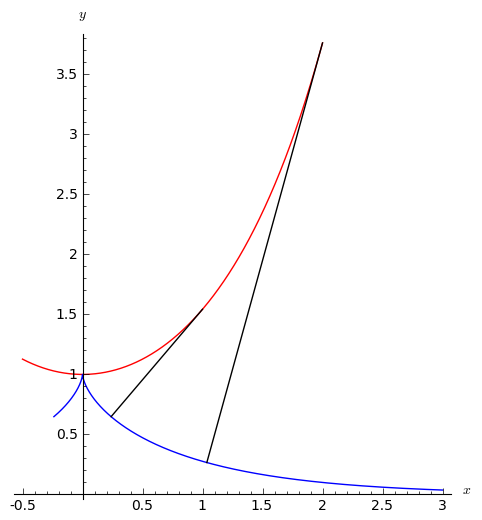
\includegraphics[height=3in]{picturebook/ch1sec2/ex1-2-16c}
\caption{The tractrix is the involute of the catenary.}
\end{figure}
\clearpage
\item[d.] First, let us show that the curve $\beta(s)$ described in the exercise 
is an evolute of $\alpha$. Let us use the Frenet notations for $\alpha$. By 
differentiating,
\[
\beta'(s) = T(s)  - \dfrac{\kappa'}{\kappa^2} N - \dfrac{1}{\kappa}(-\kappa T ) 
 = - \dfrac{\kappa'}{\kappa^2} N .
\]
This means that the tangent to $\beta$ is proportional to $N$, and hence 
perpendicular to the tangent to $\alpha$.  Also, it shows that the speed of 
$\beta$ is proportional to $\kappa'/\kappa^2$. Thus, $\beta$ is regular exactly 
when $\kappa' \neq 0$.  We need to show that $\alpha(s)$ lies on the tangent line 
to $\beta$ at $\beta(s)$.  Since the tangent to $\beta$ is proportional to the 
normal to $\alpha$, the defining equation realizes this. \\

Now, suppose $\beta$ is an evolute of the unit speed curve $\alpha$. Then $\alpha$ 
is an involute of $\beta$. Hence, (1) $\alpha(s)$ lies on the tangent line to 
$\beta$ at $\beta(s)$; and (2) the tangents at corresponding points are orthogonal. 
Note that the arclength parameter $s$ is likely not the arclength parameter of $\beta$.

By the first condition, $\alpha(s) = \beta(s) + \lambda(s)T_{\beta}(s)$. We 
differentiate this to find
\begin{equation}\label{eq:ex1-2-16--eq1}
T_{\alpha} = \beta'(s) + \lambda' T_{\beta} + \lambda T_{\beta}' 
 = (\upsilon_{\beta} + \lambda') T_{\beta} 
  + \lambda \upsilon_{\beta}\kappa_{\beta} N_{\beta} .
\end{equation}
By the second condition and the fact that $\{T_{\beta}, N_{\beta} \}$ is an 
orthonormal basis, we deduce that $\upsilon_{\beta} + \lambda'=0$. Hence 
$T_{\alpha} = \lambda \upsilon_{\beta}\kappa_{\beta}N_{\beta}$. Therefore, by 
the same kind of arguments about the pair of orthonormal bases associated to 
our curves that we keep reusing,
$T_{\beta} = a N_{\alpha}$, where $a = \pm 1$.
If we differentiate this, we see $T_{\beta}'(s) = -a\kappa_{\alpha} T_{\alpha}$. 
So substitute this information into equation (\ref{eq:ex1-2-16--eq1}) and find
\[
T_{\alpha} = 0 T_{\beta} + \lambda(-a\kappa_{\alpha}) T_{\alpha}.
\]
This implies that $\lambda = -\dfrac{1}{a\kappa_{\alpha}}$. Therefore,
\[
\alpha(s) = \beta(s) - \dfrac{1}{a\kappa_{\alpha}}(a N_{\alpha}).
\]
Which means
\[
\beta(s) = \alpha(s) + \dfrac{1}{\kappa_{\alpha}(s)} N_{\alpha}(s) .
\]
This completes the exercise.
\end{itemize}
\end{proof}

\clearpage
%%%%%%%%%%%%%%%%%%%%%%%%%%%%%%%%%%%



\begin{exercise}
Find the involute of the cycloid $\alpha(t) = (t+\sin t , 1 - \cos t)$, 
$t \in [-\pi, \pi]$, using $t=0$ as your starting point. Give a geometric 
description of your answer.
\end{exercise}

\begin{proof}[Solution]
If $\alpha$ were arclength parametrized, then we know that we must have 
$\beta(s) = \alpha(s) - s T(s)$. Rather than worry about reparametrizing 
our curve, let us instead realize that the arclength from $t=0$ is 
$s = \int_0^t \upsilon(u) \, du$, so that
\[
\beta(t) = \alpha(t) - \left( \int_0^t \upsilon(u) \, du \right) T(t) .
\]
This is much easier to compute directly, which we now do.
\begin{align*}
\alpha'(t) & = (1+\cos(t), \sin(t) ) \\
\upsilon(t) & = || \alpha'(t) || = 2 \cos(t/2) \\
s & = \int_0^t \upsilon(u) \, du = 4\sin(t/2) \\
\mbox{so} & \\
\beta(t) & = \dots = ( t -\sin(t) , \cos(t) - 1 ) .
\end{align*}
The pretty thing is that this is another cycloid!
\end{proof}

\begin{figure}[h]
\centering
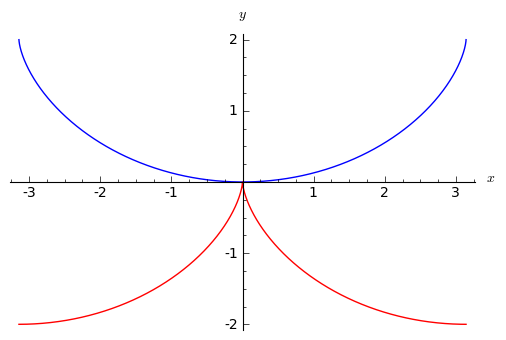
\includegraphics[height=2.5in]{picturebook/ch1sec2/ex1-2-17}
\caption{The involute of the blue cycloid is the red cycloid.}
\end{figure}



\clearpage

%%%%%%%%%%%%%%%%%%%%%%%%%%%%%%%%%%%

\begin{exercise}
Suppose that $\alpha$ is a generalized helix with axis in the direction $\mathbf{A}$. 
Let $\beta$ be the curve obtained by projecting $\alpha$ onto a plane orthogonal to 
$\mathbf{A}$. Prove that the principal normals of $\alpha$ and $\beta$ are parallel
at corresponding points and calculate the curvature of $\beta$ in terms of the 
curvature of $\alpha$.
\end{exercise}

\begin{proof}[Solution]
It would be fun to just assume, without loss of generality, that $A$ is the unit vector
in the $z$ direction and that we are projecting into the $z=0$ plane, but let's not so 
we can practice working with coordinate-free vector analysis.

Take a unit vector $A$ as the direction of the axis. The plane onto which we project 
will then consist of all vectors $X$ such that $A\cdot X = c$, where $c$ is some 
fixed number. 

We'll assume that $\alpha$ is a unit-speed curve with arclength parameter $s$. Our 
first task is to come up with a reasonable description for $\beta$. By construction,
the difference between $\alpha(s)$ and its projection $\beta(s)$ must be some 
multiple of $A$. So, $\beta(s) = \alpha(s) + \lambda(s) A$ for some function 
$\lambda(s)$. But to lie in the chosen plane, we must have $\beta(s) \cdot A = c$. 
If we put these conditions together, we learn that
\[
c = \left[ \alpha(s) + \lambda(s)A\right ]\cdot A = \alpha(s)\cdot A + \lambda
\]
So $\lambda(s) = c - \alpha(s)\cdot A$, which means that we can describe $\beta(s)$:
\[
\beta(s) = \alpha(s) + \left[ c - \alpha(s)\cdot A\right] A
\]
It is important to remember that $A$ is a constant vector, $C$ is a constant scalar,
and $\beta(s)$ is not necessarily parameterized by arclength.

Before we get going too far, let's recall that the hypothesis that $\alpha$ is a
generalized helix with axis direction $A$ means that $T_{\alpha} \cdot A = d$ is
a constant.

Now, we would like to compute the tangent, normal, and curvature of $\beta$, perhaps 
in terms of those of $\alpha$. We start by taking some derivatives and seeing what
we can figure out. Let's use primes to denote derivatives with respect to $s$.
\[
\begin{split}
\beta'(s) & = \alpha'(s) - \left[\alpha'(s) \cdot A \right] A \\
 & = T_{\alpha}(s) - \left[ T_{\alpha}(s)\cdot A \right] A \\
 & = T_{\alpha}(s) - d A
\end{split}
\]
Let's find the speed $\upsilon_{\beta}$ of $\beta$:
\[
\begin{split}
\upsilon_{\beta}^2 & = \beta'(s) \cdot \beta'(s) \\
 & = ( T_{\alpha}(s) - d A) \cdot (T_{\alpha}(s) - d A) \\
 & = T_{\alpha} \cdot T_{\alpha} - 2d T_{\alpha}\cdot A + d^2 A\cdot A \\
 & = 1 - 2d^2 + d^2 = 1-d^2.
\end{split}
\]
Most importantly, we see that the speed $||\beta'|| = \upsilon_{\beta} = \sqrt{1-d^2\, }$ is 
constant! The second derivative of $\beta$ is
\begin{equation}
\label{eq:ex1-2-18-1}
\beta''(s) = T'_{\alpha}(s) - 0 = \kappa_{\alpha}(s) N_{\alpha}(s)
\end{equation}
But as Shifrin computed near Proposition 2.2, the general expression for $\beta''$ is
\begin{equation}\label{eq:ex1-2-18-2}
\begin{split}
\beta''(s) &= \upsilon_{\beta}'(s) T_{\beta}(s) 
 + \kappa_{\beta}(s) \upsilon_{\beta}^2 N_{\beta}(s) \\
 & = \kappa_{\beta}(s) (1-d^2) N_{\beta}(s)
 \end{split}
\end{equation}
Setting equations (\ref{eq:ex1-2-18-1}) and (\ref{eq:ex1-2-18-2}) equal to each 
other, we learn that
\[
\kappa_{\alpha}(s) N_{\alpha}(s) = \kappa_{\beta}(s) (1-d^2) N_{\beta}(s).
\]

That means that the principal normal vectors for $\alpha$ and $\beta$ are parallel to 
each other at corresponding points. Further, since the principal normal vectors are 
both unit vectors, we see that
\[
\kappa_{\beta}(s) = \dfrac{\kappa_{\alpha}(s)}{1-d^2},
\]
where $d = T_{\alpha} \cdot A = \cos(\theta)$, for $\theta$ the constant angle between
the tangent to $\alpha$ and the axis $A$. 

Just for fun, we can observe that
\[
1-d^2 = 1-\cos^2(\theta) = \sin^2(\theta)
\]
is the square of the speed of $\beta$, too. This makes some sense: 
as $\theta \rightarrow \pi/2$, the curve $\alpha$ gets closer and closer to lying in 
a plane parallel to the one we have chosen, and hence the curves $\alpha$ and $\beta$ 
become very similar, so the two curvatures should be very similar. 
\end{proof}

\clearpage


%%%%%%%%%%%%%%%%%%%%%%%%%%%%%%%%%%%

\begin{exercise}
Let $\alpha$ be a curve parametrized by arclength with $\kappa,\tau \neq 0$.
\begin{itemize}
\item[a.] Suppose $\alpha$ lies on the surface of a sphere centered at the origin. Prove that
\begin{equation}\label{sphere-curve-ode}
\dfrac{\tau}{\kappa} + \left(\dfrac{1}{\tau} \left(\dfrac{1}{\kappa}\right)' \right)' =0
\end{equation}

\item[b.] Prove the converse: If $\alpha$ satisfies the differential equation 
(\ref{sphere-curve-ode}), then $\alpha$ lies on the surface of some sphere.
\end{itemize}
\end{exercise}

\begin{proof}[Solution] We'll take up the two parts independently.
\begin{itemize}
\item[a.] Since $\alpha$ lies on a sphere, we know that $||\alpha||$ is a constant. 
Since $T, N, B$ always forms an orthonormal basis, we can write
\[
\alpha = \lambda T + \mu N + \nu B
\]
for some functions $\lambda, \mu, \nu$.  The condition that $||\alpha||$ is constant 
can be differentiated to yield that
\begin{equation*}
\lambda \lambda' + \mu \mu' + \nu\nu' = 0.
\end{equation*}
Now differentiate the expression of $\alpha$ in terms of $T, N, B$ to find that
\begin{equation*}
T = (\lambda' - \mu \kappa) T + (\lambda \kappa + \mu' -\tau \nu) N + ( \mu \tau+ \nu') B .
\end{equation*}
Splitting out the components of this we find
\begin{align*}
\lambda' & = 1 + \mu \kappa , \\
\mu ' & = \tau \nu - \lambda \kappa , \\
\nu' & = -\mu \tau .
\end{align*}
If we use these expressions to eliminate the derivatives from our other equation, we find
\[
0 = \lambda (1+\mu \kappa) + \mu (\tau \nu - \lambda \kappa) + \nu (-\mu\tau) = \lambda.
\]
The fact that $\lambda = 0$ simplifies the triplet of differential equations greatly! 
We learn that  $\mu = \dfrac{-1}{\kappa}$ from the first, and then from the second that
$ \left( \dfrac{-1}{\kappa}\right)' = \tau \nu -0$, so that $\nu = 
-\dfrac{1}{\tau}\left(\dfrac{1}{\kappa}\right)'$. Now, finally the third differential 
equation is equivalent to
\[
\mu \tau + \nu' = \dfrac{\tau}{\kappa} 
+ \left(\dfrac{1}{\tau} \left(\dfrac{1}{\kappa}\right)' \right)' =0 .
\]
\clearpage
\item[b.]  Now suppose that equation (\ref{sphere-curve-ode}) holds. Motivated by what 
we learned in the last problem, we first consider the curve
\[
P(s) = \alpha(s) + \dfrac{1}{\kappa(s)} N(s) 
+ \dfrac{1}{\tau(s)}\left( \dfrac{1}{\kappa(s)}\right)' B(s) .
\]
This is our candidate for the center of the sphere. Our first goal is to see that it is 
actually a point. So we check that
\[
\begin{split}
P' &= T + \left(\dfrac{1}{\kappa}\right)' N + \dfrac{1}{\kappa} (-\kappa T + \tau B ) 
 + \left(\dfrac{1}{\tau}\left( \dfrac{1}{\kappa}\right)'\right)' B 
 + \dfrac{1}{\tau}\left(\dfrac{1}{\kappa}\right)' (-\tau N) \\
& = 0 T + 0 N + \left\{  \dfrac{\tau}{\kappa} 
 + \left(\dfrac{1}{\tau} \left(\dfrac{1}{\kappa}\right)' \right)' \right\} B = 0 .
\end{split}
\]
This means that $P(s) = P$ is really constant. It will be the center of the sphere on 
which $\alpha$ lies. To finish the exercise, we must see that $\alpha$ lies a constant 
distance from $P$. For this, note that
\[
\begin{split}
\dfrac{d}{ds} ||\alpha(s) - P||^2 = 2 T \cdot (\alpha-P) 
= 2 T \cdot ( \lambda N + \mu B) = 0.
\end{split}
\]
This completes the exercise.
\end{itemize}
\end{proof}

\clearpage

%%%%%%%%%%%%%%%%%%%%%%%%%%%%%%%%%%%

\begin{exercise}
Two distinct parametrized curves $\alpha$ and $\beta$ are called \emph{Bertrand mates} 
if for each $t$, the normal line to $\alpha$ at $\alpha(t)$ equals the normal line to 
$\beta$ at $\beta(t)$. Suppose that $\alpha$ and $\beta$ are Bertrand mates.
\begin{itemize}
\item[a.] If $\alpha$ is arclength-parametrized, show that $\beta(s) = \alpha(s) + r(s) N(s)$ 
and $r(s) = \mbox{const}$. Thus, corresponding points of $\alpha$ and $\beta$ are a constant 
distance apart.
\item[b.] Show that, moreover, the angle between the tangent vectors to $\alpha$ and $\beta$ 
at corresponding points is constant.
\item[c.] Suppose that $\alpha$ is arclength-parametrized and $\kappa\tau \neq 0$. Show that 
$\alpha$ ha a Bertrand mate $\beta$ if and only if there are constants $r$ and $c$ so that 
$r\kappa + c\tau =1$.
\item[d.] Given $\alpha$, prove that if there is more than one curve $\beta$ so that 
$\alpha$ and $\beta$ are Bertrand mates, then there are infinitely many such curves $\beta$ 
and this occurs if and only if $\alpha$ is a circular helix.
\end{itemize}
\end{exercise}

\begin{proof}[Solution]$ \ $ \\
\begin{itemize}
\item[a.] Suppose that $\beta$ is a Betrand mate for $\alpha$. Since $\beta(s)$ lies on 
the normal line to $\alpha$ at $\alpha(s)$, there is some function $r(s)$ such that 
$\beta(s) = \alpha(s) + r(s) N(s)$. Differentiating, we find
\[
\upsilon_{\beta} T_{\beta}(s)  = T_{\alpha}(s) + r'(s) N_{\alpha}(s) 
+ r(s) \left( -\kappa_{\alpha}(s) T_{\alpha}(s) + \tau(s) B_{\alpha}(s) \right)  .
\]
By the Bertrand condition, we must have that $T_{\beta}$ is perpendicular to 
$N_{\alpha}$, so
\[
0 = T_{\beta} \cdot N_{\alpha} = \dfrac{r'(s)}{\upsilon_{\beta}}.
\]
Hence $r'(s) = 0$, so $r(s)=r$ is constant. Also, we gather for later use that
\[
\dfrac{d}{ds}\beta = (1- r \kappa_{\alpha}(s) )T_{\alpha}(s) 
+ r\tau_{\alpha}(s) B_{\alpha}(s).
\]
So the speed of $\beta$ satisfies
\[
\upsilon_{\beta}^2 = (1-r\kappa_{\alpha})^2 + r^2 \tau_{\alpha}^2.
\]


\item[b.] The angle between (unit) tangent vectors is the number $\theta$ so that 
$\cos\theta = T_{\alpha}\cdot T_{\beta}$, so this follows from the observation that
\[
\left( T_{\alpha} \cdot T_{\beta} \right)' = T_{\alpha} \cdot(\upsilon_{\beta}\kappa_{\beta}N_{\beta}) 
+ (\kappa_{\alpha} N_{\alpha}) \cdot T_{\beta} = 0 ,
\]
since the normal lines of the two curves coincide.

\item[c.] First, suppose that $\alpha$ and $\beta$ are Bertrand mates.  We showed 
in the last part that $T_{\alpha} \cdot T_{\beta} = c$ is a constant. We next 
compute that
\[
\begin{split}
1- r \kappa_{\alpha} & = T_{\alpha} \cdot \dfrac{d\beta}{ds} \\
	& = T_{\alpha} \cdot (\upsilon_{\beta} T_{\beta} ) \\
	& = c \upsilon_{\beta} \\
	& = c \left( (1-r\kappa_{\alpha})^2 + r^2 \tau_{\alpha}^2 \right)^{1/2}
\end{split}
\]
With some manipulation, this can be massaged into the form
\[
1 = r \kappa_{\alpha} + c' \tau_{\alpha}
\]
where $c' = r c / \sqrt{1-c^2\,}$. \\

Now suppose that the equation holds for a unit speed curve $\alpha$. We must show 
that $\alpha$ has a Bertrand mate. Let $\beta(s) = \alpha(s) + r N(s)$.
Then, as before,
\[
\upsilon_{\beta} T_{\beta} = \dfrac{d\beta}{ds} = (1 - r\kappa) T + r\tau B
\]
Since $T, B$ are an orthonormal set, we see that
\[
\begin{split}
\upsilon_{\beta}^2 & =  (1-r\kappa)^2 + (r\tau)^2 \\
	& = (c\tau)^2 + (r\tau)^2 \\
	& = \tau^2 (c^2+r^2) .
\end{split}
\]
Therefore, the above equation for $T_{\beta}$ can be rewritten as
\[
|\tau| \sqrt{c^2+r^2} T_{\beta} = \tau (cT_{\alpha} + r B_{\alpha} ).
\]
From which we learn that
\[
T_{\beta} = \pm \left( \dfrac{c}{\sqrt{c^2+r^2}} T_{\alpha} 
+ \dfrac{r}{ \sqrt{c^2+r^2} } B_{\alpha} \right) .
\]
And now by differentiating,
\[
\upsilon_{\beta} \kappa_{\beta} N_{\beta} = 
\pm \left(  \dfrac{ (c-r) \kappa_{\alpha} }{ \sqrt{c^2+r^2} } \right) N_{\alpha}.
\]
This shows that the normal to $\beta$ is parallel or anti-parallel to the normal to 
$\alpha$, so the curves are Bertrand mates.


\item[d.]  Now suppose that the curve $\alpha$ has two Bertrand mates, $\beta_1$ and 
$\beta_2$. By the last part of the exercise, there are distinct pairs of constants 
$c_1,  r_1$ and $c_2, r_2$ such that
\[
1 = r_1 \kappa + c_1 \tau = r_2 \kappa + c_2 \tau .
\]
This implies that $ (r_1 - r_2) \kappa = (c_2 - c_1) \tau $. So the curvature and 
torsion are proportional. Since the pairs of constants are distinct, at least one 
of the $r_1-r_2$ or $c_1-c_2$ is non-zero. Without loss of generality, assume that 
$r_1-r_2 \neq 0$. Then we have
\begin{equation*}\label{eq:ex1-2-19}
1 = r_1 \kappa + c_1 \left( \dfrac{c_2 - c_1}{r_1-r_2}\right) \kappa .
\end{equation*}
This implies that $\kappa$ is a constant, and hence $\tau$ is a constant, too.  
Thus $\alpha$ is a circular helix.

Now, if $\alpha$ is a circular helix, we know that $\kappa$ and $\tau$ are constants, 
and there is another constant $a$ so that $\tau = a\kappa$. We may now find 
infinitely many solutions $(r,c)$ to the equation
\[
1 = r\kappa + c\tau = (r+ca) \kappa
\]
by allowing $c$ to vary freely and taking $r = -ac + 1/\kappa$. By the last part 
of the exercise, each of these choices leads to a Bertrand mate of the circular 
helix, and since $r$ is different for each, the curves are clearly distinct.
\end{itemize}
\end{proof}

\vspace{.5cm}

%%%%%%%%%%%%%%%%%%%%%%%%%%%%%%%%%%%

\begin{exercise}
Suppose that $\alpha$ and $\beta$ are Bertrand mates. Prove that the torsion 
of $\alpha$ and the torsion of $\beta$ at corresponding points have constant product.
\end{exercise}

\begin{proof}[Solution]
\todo[inline]{Solve this problem.}
\end{proof}

\vspace{.5cm}

%%%%%%%%%%%%%%%%%%%%%%%%%%%%%%%%%%%

\begin{exercise}
Suppose that $Y$ is a $\mathcal{C}^2$ vector function on $[a,b]$ with $||Y||=1$ 
and $Y$, $Y'$ and $Y''$ everywhere linearly independent. For any non-zero 
constant $c$, define $\alpha(t)  = c\int_a^t (Y(u) \times Y'(u)) \, du$, $t \in [a,b]$. 
Prove that the curve $\alpha$ has constant torsion $1/c$.
\end{exercise}

\begin{proof}[Solution]

\end{proof}

\vspace{.5cm}

%%%%%%%%%%%%%%%%%%%%%%%%%%%%%%%%%%%

\begin{exercise}
Suppose that $Y$ is a $\mathcal{C}^2$ arclength-parametrized curve on the unit 
sphere. For any non-zero constant $a$ and $0 < \theta \leq \pi/2$, define
\[
\alpha(t)  = 
a \left( \int_0^t Y(s) \, ds + \cot \theta \int_0^t (Y(s) \times Y'(s))\, ds\right) .
\]
Show that the curve $\alpha$ has a Bertrand mate.
\end{exercise}

\begin{proof}[Solution]

\end{proof}

\clearpage

%%%%%%%%%%%%%%%%%%%%%%%%%%%%%%%%%%%

\begin{exercise} $\ $\\
\begin{itemize}
\item[a.] Let $\alpha$ be an arclength-parametrized plane curve. We create a 
``parallel'' curve $\beta$ by taking $\beta = \alpha + \varepsilon N$ for some 
fixed small positive value of $\varepsilon$. Explain the terminology and express 
the curvature of $\beta$ in terms of $\varepsilon$ and the curvature of $\alpha$.
\item[b.] Now let $\alpha$ be an arclength-parametrized space curve. Show that 
we can obtain a ``parallel'' curve $\beta$ by taking 
$\beta = \alpha + \varepsilon\left( \cos\theta N + \sin\theta B\right)$. 
How many such parallel curves are there?
\item[c.] Sketch such a parallel curve for a circular helix $\alpha$.
\end{itemize}
\end{exercise}

\begin{proof}[Solution] One part at a time\dots
\begin{itemize}
\item[a.] We start with the plane curve. Let $s$ be the arclength parameter 
of $\alpha$. Note that $\upsilon_{\beta} T_{\beta} = \dfrac{d\beta}{ds} = 
T_{\alpha} + \varepsilon ( -\kappa_{\alpha} T_{\alpha} ) = 
(1-\varepsilon\kappa_{\alpha}) T_{\alpha}$, so the curves have parallel tangent 
vectors and the speed of $\beta$ with respect to $s$ is $\upsilon_{\beta}(s) = 
|1-\varepsilon\kappa_{\alpha}(s) |$. If the tangent vectors are parallel, we must 
have $T_{\beta} = T_{\alpha}$. Now to find the curvature, we differentiate
\[
\upsilon_{\beta} \kappa_{\beta} N_{\beta} = \dfrac{d}{ds} T_{\beta} = T_{\alpha}' 
= \kappa_{\alpha} N_{\alpha}.
\]
Since the normal vectors are both unit vectors, we read off that the curvature of 
$\beta$ is
\[
\kappa_{\beta} = \dfrac{\kappa_{\alpha}}{\upsilon_{\beta} } 
= \dfrac{\kappa_{\alpha}}{1-\varepsilon\kappa_{\alpha}} .
\]

\item[b.] Now consider a unit-speed space curve and the associated $\beta$ as 
in the statement. Differentiating the defining equation for $\beta$ we find
\[
\begin{split}
\dfrac{d\beta}{ds} & = T_{\alpha} 
 + \varepsilon( -\sin(\theta) \theta') N_{\alpha} 
 + \varepsilon\cos(\theta) (-\kappa T_{\alpha} + \tau B_{\alpha}) \\
& \qquad  + \varepsilon\cos(\theta) \theta' B_{\alpha} 
 + \varepsilon\sin(\theta) ( -\tau N_{\alpha})  \\
& = (1-\varepsilon\kappa\cos(\theta)) T_{\alpha} 
 - \varepsilon\sin(\theta) (\theta' + \tau) N_{\alpha} 
 + \varepsilon\cos(\theta) ( \tau + \theta') B_{\alpha} .
\end{split}
\]
So our curve $\beta$ will be parallel to $\alpha$ when $\theta' + \tau = 0$, that is, 
when $\theta(s) = -\int_{s_0}^s \tau(u) \, du$. There is a whole one parameter family  
of these curves corresponding to the choice of starting point $s_0$. Since this is like 
a phase shift in the trig functions, we essentially get a circle's worth of parallel 
curves.

\clearpage

\item[c.] The arclength parametrized helix is
\[
\alpha(s) = \left( a \cos(s/c), a \sin(s/c) , \dfrac{bs}{c} \right),
\]
where $c = \sqrt{a^2+b^2}$.  We have computed that the torsion of this curve is 
$\tau = \dfrac{b}{c^2}= \dfrac{b}{a^2+b^2}$. So if we choose $s_0=0$ as our base point, 
then
\[
\theta = - \int_0^2 \dfrac{b}{c^2} \, ds = -\dfrac{bs}{c^2}.
\]
Following the above, then we see
\[
\begin{split}
\beta(s) = & \left(  a \cos(s/c) +\varepsilon\left[ -\cos(bs/c^2)\cos(s/c) 
  - \dfrac{b}{c}\sin(bs/c^2)\sin(s/c)\right] , \right. \\
& \qquad a \sin(s/c) +\varepsilon \left[ \cos(bs/c^2)\sin(s/c) + \dfrac{b}{c}\sin(bs/c^2)\cos(s/c)\right] , \\
& \qquad \left. \dfrac{bs}{c} - \varepsilon\dfrac{a}{c}\sin(bs/c^2)  \right) .
\end{split}
\]
The helix goes around one turn as $s$ runs from $0$ to $2\pi c = 2\pi\sqrt{a^2+b^2}$. 
The parallel curve $\beta$ spins around this curve and goes around it one full turn 
in the normal plane as $s$ runs from $0$ to $2\pi\sqrt{a^2+b^2}/b$.

\todo[inline]{insert picture here}

\end{itemize}
\end{proof}

\clearpage
%%%%%%%%%%%%%%%%%%%%%%%%%%%%%%%%%%%

\begin{exercise}
Suppose $\alpha$ is an arclength-parametrized curve, 
$P = \alpha(0)$, and $\kappa(0) \neq 0$. Use Proposition 2.6 to establish the following:
\begin{itemize}
\item[a.] Let $Q = \alpha(s)$ and $R = \alpha(t)$. Show that the plane spanned by 
$P, Q$ and $R$ approaches the osculating plane of $\alpha$ at $P$ as $s,t\rightarrow 0$.
\item[b.] The \emph{osculating circle} at $P$ is the limiting position of the circle 
passing through $P, Q$ and $R$ as $s,t \rightarrow 0$. Prove that the osculating circle 
has center $Z = P + (1/\kappa(0)) N(0)$ and radius $1/\kappa(0)$.
\item[c.] The \emph{osculating sphere} at $P$ is the limiting position of the sphere 
through $P$ and three neighboring points on the curve, as the latter points tend to $P$ 
independently. Prove that the osculating sphere has center
\[
Z= P + \left( \dfrac{1}{\kappa(0)}\right) N(0) + \left(  \dfrac{1}{stuff...}  \right) B(0)
\]
and radius
\[
\sqrt{  \left( \dfrac{1}{\kappa(0)}\right)^2  + \left(  \dfrac{1}{stuff...}  \right)^2 } .
\]
\item[d.] How is the result of part c related to Exercise 18?
\end{itemize}
\end{exercise}

\begin{proof}[Solution]
\item[a.] Well, we did this in class and I made a handout\dots

\item[b.] Suppose that $P = \alpha(0)$, $Q= \alpha(s)$ and $R=\alpha(t)$ are three 
points on the curve.

\end{proof}

\vspace{.5cm}

%%%%%%%%%%%%%%%%%%%%%%%%%%%%%%%%%%%

\begin{exercise}$\ $\\
\begin{itemize}
\item[a.] Suppose that $\beta$ is a plane curve and $C_s$ is the circle centered 
at $\beta(s)$ with radius $r(s)$. Assuming $\beta$ and $r$ are differentiable 
functions, show that the circle $C_s$ is contained inside the circle $C_t$ whenever 
$t\geq s$ if and only if $||\beta'(s)|| \leq r'(s)$ for all $s$.
\item[b.] Let $\alpha$ be an arclength-parametrized plane curve and suppose $\kappa$ 
is a decreasing function. Prove that the osculating circle at $\alpha(s)$ lies inside 
the osculating circle at $\alpha(t)$ whenever $t\geq s$.
\end{itemize}
\end{exercise}

\begin{proof}[Solution]

\end{proof}

\vspace{.5cm}

%%%%%%%%%%%%%%%%%%%%%%%%%%%%%%%%%%%

\begin{exercise}
Suppose that the front wheel of a bicycle follows the arclength-parametrized plane 
curve $\alpha$. Determine the path $\beta$ of the rear wheel, $1$ unit away.
\end{exercise}

\begin{proof}[Solution]

\end{proof}

\vspace{.5cm}

%%%%%%%%%%%%%%%%%%%%%%%%%%%%%%%%%%%

\end{document}
